% time values for run11, run14 and run15
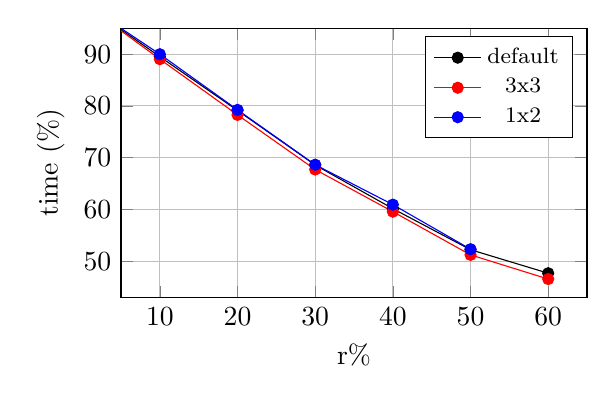
\begin{tikzpicture}
\begin{axis}[
    title={},
    height=5cm,
    width=7.5cm,
    xlabel={r\%},
    ylabel={time (\%)},
    xmin=5, xmax=65,
    ymin=43, ymax=95,
    xtick={10,20,30,40,50,60},
    ytick={50,60,70,80,90},
    legend pos=north east,
    xmajorgrids=true,
    ymajorgrids=true,
    legend style={font=\footnotesize}
]

\addplot[
    color=black,
    mark=*
    ]
    coordinates {
    (0,100)(10,89.50)(20,79.11)(30,68.57)(40,60.14)(50,52.21)(60,47.67)
    };
    
\addplot[
    color=red,
    mark=*
    ]
    coordinates {
    (0,100)(10,89.02)(20,78.26)(30,67.70)(40,59.56)(50,51.21)(60,46.54)
    };

\addplot[
    color=blue,
    mark=*
    ]
    coordinates {
    (0,100)(10,89.98)(20,79.23)(30,68.63)(40,60.92)(50,52.31)
    };
    
\legend{default, 3x3, 1x2}
    
\end{axis}
\end{tikzpicture}